\section{Experiment 1: Simulated Data from Multivariate Normal Distribution}

	In the first simulation experiment, we focused on an ideal setting where data come from a known multivariate normal 
	distribution and imputation is required to estimate the means, variances, and covariances of six items with 
	missing values.
	We investigated the relative performance of the methods described above across a set of conditions defined by two 
	experimental factors: the number of columns in the dataset $p$, taking values 50 or 500; 
	and the proportion of \emph{per} variable missing cases $pm$, taking values 0.1 or 0.3.
	Table \ref{tab:condExp1} summarizes the four crossed conditions.
	Data with sample size $n=200$ were independently generated $S = 1,000$ times for each condition.
	For each $s$-th replicate, missing values were imposed and then all the missing data treatment methods described above
	were used to obtain estimates of the item means, variances, and covariances.

\begin{table}
	\centering
	\begin{tabular}{l | r | r | r | r }
		condition & label & n & p & pm \\
		\hline
		1 & low-dim-low-pm   & 200 & 50  & .1 \\
		2 & high-dim-low-pm  & 200 & 500 & .1 \\
		3 & low-dim-high-pm  & 200 & 50  & .3 \\
		4 & high-dim-high-pm & 200 & 500 & .3 \\
	\end{tabular}
	\caption{\label{tab:condExp1}Summary of conditions for Experiment 1.}
\end{table}

%\FloatBarrier

\subsection{Simulation Study Procedure}

\subsubsection{Data Generation}
	At every replication, a data matrix $\bm{Z}_{n \times p}$ was generated according to a multivariate normal model 
	centered around a mean of 0 with a covariance matrix $\bm{\Sigma}_0$, with diagonal elements (variances) equal to 1.
	The off-diagonal elements of $\bm{\Sigma}_0$ were used to define three blocks of variables: 
	the first five variables were highly correlated among themselves ($\rho = .6$);
	variables 6 to 10 were weakly correlated with variables in block 1 and among themselves ($\rho = .3$), 
	and all the remaining $p-10$ variables were uncorrelated.
	Items were rescaled to have mean of 5.

\subsubsection{Missing Data Imposition} \label{sub_missing}

	Missing values were imposed on six items in $\bm{Z}$: three variables in the block of
	highly correlated variables ($z_j$ with $j = 1,2,3$), and three in the block of lowly correlated variables ($z_j$ 
	with $j = 6,7,8$).
	Item non-response was imposed by sampling from a Bernoulli distribution with individual missing probabilities 
	defined by 
%
	\begin{equation} \label{eqn:rm}
		p_{miss} = p(z_{i,j} = miss | \tilde{Z}) = \frac{ exp(\gamma_0 + \tilde{Z}_{i}\bm{\gamma}) }
								{ 1 + exp(\gamma_0 + \tilde{Z}_{i}\bm{\gamma}) }
	\end{equation}
%
	where $z_{i,j}$ is the $i$-th subject's response on the $j$-th variable target of missing data imposition, 
	$\tilde{Z}_{i}$ is a vector of responses to the set of predictors involved in the missing data mechanism 
	for the $i$-th individual, $\gamma_0$ is an intercept parameter, and $\bm{\gamma}$ is a vector of slope 
	parameters for the linear term.
	$\tilde{Z}$ was specified to include two fully observed variables from the highly correlated set, and two 
	from the lowly correlated set ($z_r$ with $r = 4,5,9,10$).
	The probability of observing a response on a target variable did not depend on the variable itself, 
	to avoid imputation under MNAR.
	Furthermore, when all the features in the data are provided to the MI procedures, the predictors in $\tilde{Z}$ 
	are allowed to be part of the imputation models and the MAR assumption can be met.
	All slopes in $\bm{\gamma}$ were fixed to 1, while the value of $\gamma_0$ was chosen with an optimization 
	algorithm that minimized the difference between the actual and desired proportion of missing values.

\subsubsection{Imputation}
	
	Missing values were treated with all the methods described in Section 2.
	Convergence of the imputation models was assessed in a preprocessing step by observing trace plots.
	The imputation algorithms were considered to have converged after 50 iterations, after which 10 imputed data 
	sets were stored and used for the subsequent standard complete-data analysis and pooling.
	The only exception was blasso, which required approximately 2,000 iterations for convergence.

	The ridge penalty used in the bridge algorithm was fixed across iterations.
	The value used in the simulation was determined by means of cross-validation in a preprocessing phase.
	The ridge penalty values $10^{-1}, 10^{-2}, ..., 10^{-8}$ were used to impute data with bridge
	and we selected the value that resulted in the smallest average Fraction of Missing Information (FMI)
	\citep[eq. 3.1.10]{rubin:1987} across the analysis model parameters.
		
	Both IURR and DURR could have been specified with a variety of penalty parameters.
	For example, one could use any of the following: ridge penalty \citep{hoerlKennard:1970}, lasso penalty 
	\citep{tibshirani:1996}, elastic net penalty \citep{zouHastie:2005}, adaptive lasso \citep{zou:2006}.
	In this study, we specified the lasso penalty for regularization as it is computationally efficient, 
	and it performed well for imputation in \cite{zhaoLong:2016} and \cite{dengEtAl:2016}.
	A 10-fold cross-validation procedure was used at every iteration of DURR and IURR to choose the penalty parameter.

	For blasso, in order to maintain consistency with previous research, the hyper-parameters in equations 
	\eqref{eqn:sigprior}, \eqref{eqn:tauprior}, and \eqref{eqn:rhoprior} were specified as in \cite{zhaoLong:2016}: 
	$(a,b)=(0.1, 0.1)$, $(r,s)=(0.01, 0.01)$, and $(g,h)=(1,1)$.
	In the MI-PCA algorithm, enough components were extracted to explain 50\% of the total variance in the data.
	To impute data with the single imputation random forest approach we used the missForest R package 
	\citep{missForest} implementing algorithm 1 proposed by \cite{stekhovenBuhlmann:2011}.
	The stopping criterion for the missForest algorithm was usually met within the first 10 iterations, 
	but to make a conservative choice we fixed the maximum number of iterations to 20.
	\cite{stekhovenBuhlmann:2011} showed that increasing the number of trees grown in each forest has 
	stagnating effects on the imputation error while linearly increasing the computation time.
	In their paper, the authors recommend growing 100 trees per forest, which offers a good compromise 
	between imputation precision and computation time.
	Therefore, we used this value in our study.

\subsubsection{Analysis}
	The substantive model of interest in Experiment 1 was a saturated model that estimated means,
	variances, and covariances of the six variables with missing values.
	This resulted in estimating six means, six variances, and 15 covariances.

\subsection{Comparison Criteria} \label{criteria}

	We compared methods in terms of bias and confidence interval coverage.

	\paragraph{Bias}

	For a given parameter of interest $\theta$ (e.g., mean of item 1, variance of item 2), we used the 
	Percent Relative Bias (PRB) to quantify the estimation bias introduced by the imputation procedures:
%
	\begin{equation} \label{eqn:prb}
		PRB = \frac{\bar{\hat{\theta}} - \dot{\theta}}{\dot{\theta}} \times 100
	\end{equation}
%
	where $\dot{\theta}$ is the true value of the focal parameter defined as 
	$\sum_{s=1}^{S} \hat{\theta}_{s}^{GS}/S$
	, with
	$\hat{\theta}_{s}^{GS}$ 
	being the Gold Standard parameter estimate for the $s$-th repetition. 
	The averaged focal parameter estimate under a given missing data treatment is computed as 
	$\bar{\hat{\theta}} = \sum_{s=1}^{S} \hat{\theta}_{s}/S$,
	with
	$\hat{\theta}_{s}$ being the estimate obtained after having treated the missing values in the 
	$s$-th repetition.
	Following \cite{muthenEtAl:1987}, $|\text{PRB}| > 10\%$ was considered indicative of problematic 
	estimation bias.

	\paragraph{Confidence Intervals Coverage}
	To assess the correctness of hypothesis testing, the Confidence Interval Coverage (CIC) of the true parameter
	value was defined as:
%
	\begin{equation} \label{eqn:cic}
		CIC =  \frac{ \sum_{s=1}^{S} I(\dot{\theta} \in \widehat{CI}_s ) }{S}
	\end{equation}
%
	where $\widehat{CI}_s$ is the confidence interval of the parameter estimate $\hat{\theta}_{s}$ in a given repetition, 
	and $I(.)$ is the indicator function that returns 1 if the argument is true and 0 otherwise.
	
	CICs below 0.9 are usually considered problematic for 95\% confidence intervals \cite[p. 52]{vanBuuren:2018} 
	as they imply inflated Type I error rates.
	A high coverage (e.g., 0.99) may indicate confidence intervals that are too wide, implying inflated Type II error rates.
	Therefore, Confidence Intervals were considered to show severe under-coverage (over-coverage) if they were 
	below 0.9 (above 0.99).

	Following \cite{burtonEtAl:2006}, in simulation studies, a CIC can be considered as significantly different from the 
	nominal coverage rate if it falls outside two Standard Errors of the nominal coverage probability ($SE(p)$) from the 
	nominal coverage rate.
	The standard error of nominal coverage probability is defined as $SE(p) = \sqrt{p (1-p)/S}$, with $p$ indicating the
	chosen nominal coverage probability.
	Therefore, for $S = 1000$, 95\% CI coverages ($p = 0.95$) outside the range (0.94, 0.96) were considered as significantly 
	different from the nominal coverage rate.

\subsection{Results}
	
	Both PRB and CIC were computed for all the 27 parameters in the analysis model (six means, six item variances,
	and 15 covariances).
	To summarize the results, we focus on the typical and extreme values of these measures.
	In Figures \ref{fig:exp1bias} and \ref{fig:exp1cir}, we report the average, minimum, and maximum absolute PRB 
	and CIC achieved by the missing data treatment methods for each parameter parameter type.
	In the supplementary material, we included figures reporting the raw PRB and CIC for every parameter estimate.
%
	\paragraph{Means} 
	Focusing first on the item means (top rows), the largest $|\text{PRB}|$ is below 10 percentage points for all 
	imputation methods.
	However, looking at relative performances, IURR and MI-PCA resulted in smaller bias than all other methods, 
	except MI-OP.
	In the conditions with high proportion of missing values (columns 3 and 4 in the figures), all methods showed 
	significant deviations from nominal coverage rates, with all CICs outside of the interval $(0.94, 0.96)$.
	The only exceptions was MI-PCA which showed non-significant deviations from nominal coverage for 
	almost all estimates, with both the lowest and highest CIC falling within (0.94, 0.96) in all conditions.
	The tree-based MI methods, missForest, and CC lead to CICs significantly different from nominal coverage rates
	in all conditions.
%
	\paragraph{Variances} 
	Moving to the item variances (central rows), IURR, blasso, and the MI tree-based methods resulted in the lowest
	biases across all conditions, even in the high-dim-high-pm condition.
	These low biases were mostly paired with low deviations from nominal coverage, except for the high-dim-high-pm
	condition where they resulted in significant under-coverage of the true item 
	variances (highest $CIC < 0.94$).
	Nevertheless, apart from MI-OP, blasso was the method with best coverage in this final condition.
	
	DURR showed poor performance with regard to the item variances: in all conditions but the first, it led to 
	large bias accompanied by significant CI under-coverage.
	Bridge was the only MI method showing larger bias than DURR in all the high-dimensional conditions (columns 2 and 4),
	with even the minimum $|\text{PRB}|$ exceeding the 20\% threshold.
	MI-PCA also showed poor performance with noticeable item variance bias in all conditions that became extreme in the
	high-dim-high-pm condition (column 4), where even the smallest $|\text{PRB}|$ exceeded 20\%.
	This poor performance was reflected in extreme confidence interval under-coverage of the true item variances in
	the final experimental condition.
	Finally, missForest and CC led to substantial bias and CI under-coverage for all 
	item variances, even in condition 1.
%
	\paragraph{Covariances}
	IURR performed noticeably better than most other methods, with negligible covariance bias 
	(maximum $|\text{PRB}| < 10\%$) and acceptable coverage (average $CIC \sim 0.94$) in the high-dim-low-pm 
	condition.
	However, it struggled with a large covariance bias and extreme under-coverage in the high-dim-high-pm 
	condition (average $|\text{PRB}| > 10\%$ and average $CIC < 0.90$).
	MI-PCA showed negligible bias for all the covariance estimates (with the maximum $|\text{PRB}| < 10\%$), 
	and performed as well as MI-OP in all but the high-dim-high-pm condition.
	Furthermore, MI-PCA resulted in virtually no deviation from nominal coverage, except in the last condition.
	In the high-dim-high-pm condition, MI-PCA led to negligible bias, and mild significant \emph{over}-coverage 
	of the items covariances: the average CIC was greater than 0.96, but smaller than 0.99.

	Bridge displayed low bias and acceptable coverage in the low dimensional conditions (columns 1 and 3), but 
	extreme bias and low CI coverage in all the high dimensional conditions (columns 2 and 4).
	MissForest and CC showed extreme bias and under-coverage for all the covariances (minimum $|\text{PRB}|>10\%$),
	even in condition 1.
	All other methods, including DURR, showed absolute covariance PRBs larger than the 10\% threshold in all but the 
	first condition, with persistently significant CI under-coverage of the true values.

\begin{figure}
\centering
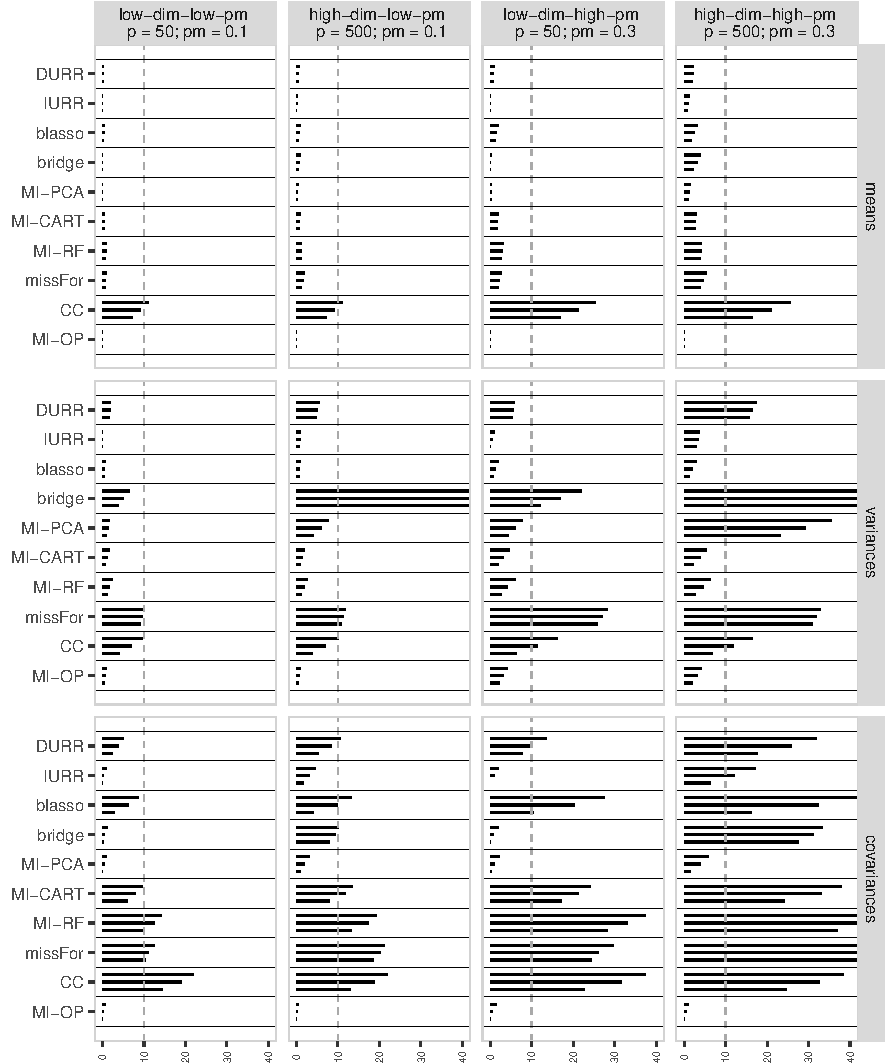
\includegraphics{\pathFIG/exp1_bias_summy.pdf}
\caption{\label{fig:exp1bias}
	Maximum, average, and minimum absolute Percent Relative Bias ($|\text{PRB}|$) for item means, variances, 
	and covariances in Experiment 1.
	For each method, the maximum, average, and minimum $|\text{PRB}|$ are reported in this order.
	}
\end{figure}

\begin{figure}
\centering
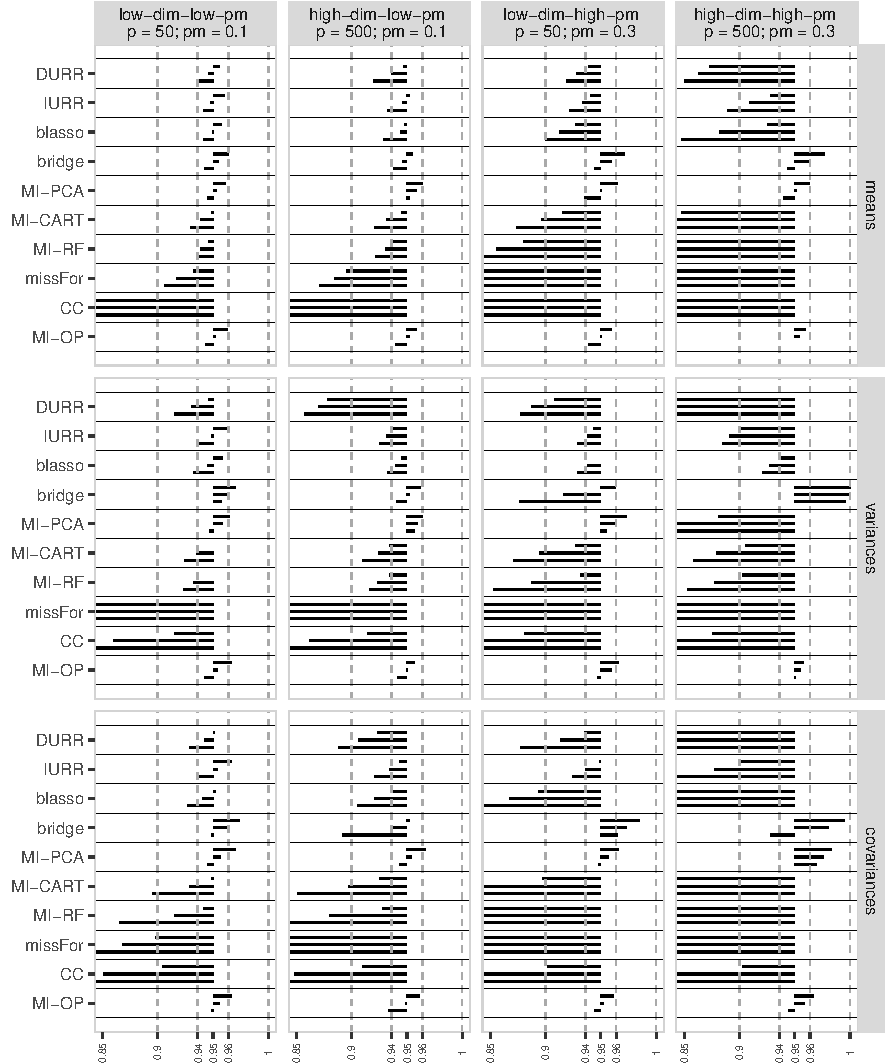
\includegraphics{\pathFIG/exp1_CI_summy.pdf}
\caption{\label{fig:exp1cir}
	Maximum, average, and minimum CIC for item means, variances, and covariances in Experiment 1.
	For each method, the maximum, average, and minimum are reported in this order.
	}
\end{figure}
	
%\FloatBarrier % stops fig:exp1cir to leave its section

